\documentclass{article}

\title{Praca magisterska, wersja robocza}
\date{2015-09-02}
\author{Hubert Guzera}



\usepackage{polski}
\usepackage[utf8]{inputenc}
\usepackage{natbib}
\usepackage{graphicx}

\begin{document}



\maketitle
\pagenumbering{gobble}

\pagenumbering{arabic}

\paragraph{Wprowadzenie} \mbox{}\\

Wal-Mart, amerykański gigant handlowy, co godzinę umieszcza w swoich bazach danych 2.5 petabajtów danych, pochodzących z blisko miliona transakcji.I nie jest wyjątkiem - przeciętna ilość danych przechowywanych przez przedsiębiorstwa w Stanach Zjednoczonych jest większa niż zbiory Biblioteki Kongresu (a te z kolei szacowane są na 235 terabajtów). W erze informacji większość z danych generowanych przez konsumentów trafia na serwery tej bądź innej firmy, czy to w formie historii transakcji, koordynatu GPS czy zdjęcia. 

Często informacje te zbierane są przypadkiem. Ze względu na prowadzenie rachunkowości, specyfikę świadczonych usług, lub też względy archiwizacyjne. Jednak wydobycie z nich \textit{wiedzy} może stanowić źródło znaczącej przewagi konkurencyjnej.  Jak wskazują Brynjolfsson, Hitt i Kim \cite{Brynjolfsson2011}, przedsiębiorstwa podejmujące decyzje na podstawie analizy dużych zbiorów danych (\textit{data driven decision making} osiągają efektywność o 5-6 proc. większą niż grupa porównawcza. Osiągają także większy zwrot z kapitału i wycenę rynkową - jednym słowe, radzą sobie lepiej. Nic więc dziwnego, że coraz częściej data analytics staje się priorytetem wśród dużych spółek. Skalę popularności business intelligence unaocznia badanie PwC \cite{PwC2014}, według którego 44 proc. CEO planuje oparcie rozwoju firmy o inwestycje w tej dziedzinie. 

Ale dzisiejsze zastosowania \textit{big data} to tylko preludium do tego, co czeka nas w przyszłości. Analiza danych w celu podejmowania decyzji menedżerskich to jedno, jednak trwający równolegle trend robotyzacji spowoduje, że w ciągu 20 lat w przedsiębiorstwie zamiast kierowców możemy zarządzać flotą autonomicznych pojazdów, a magazynierów zastąpią roboty. Fakt, że Google i Daimler już testują takie auta nie pozwala na nazwanie tego science-fiction. Według Carla Freya i Michela Osborne'a z Uniwersytetu w Oxfordzie \cite{Frey2013}, blisko 47 proc. miejsc pracy jest zagrożonych komputeryzacją. Większość z nich to zawody wykonujące rutynowe, mechaniczne czynności, ale postęp technologiczny powoduje, że na tej liście znajdują się też prace wymagające umiejętności kognitywnych i wnioskowania, jak pracownicy biurowi, analitycy czy operatorzy. 

Jeśli więc w jednej strony mamy do czynienia z flotą autonomicznych pojazdów, z a drugiej z petabajtami informacji o tym gdzie i co kupują nasi klienci, możemy znaleźć się w sytuacji, gdzie koordynacja łańcucha dostaw będzie wykraczać poza możliwości człowieka. Dla komputera, wyprognozowanie popytu na podstawie danych i zaplanowanie dostaw nie będzie żadnym problemem. Potwierdza to The McKinsey Global Institute \cite{McKinsey&Company2011}, który wskazuje, że coraz częściej maszyny będą zastępować ludzi w podejmowaniu decyzji i brać udział w sterowaniu przedsiębiorstwem. W teorii, ze względu na możliwość przeprowadzania złożonych obliczeń i analizy gigabajtów danych, decyzje te będą trafniejsze i poprawią efektywność przedsiębiorstwa. 

Niniejsza praca ma dwa główne cele. Pierwszym z nich jest zaproponoiwania jednego  z wielu możliwych algorytmów optymalizacji przedsiębiorstwa poprzez wykorzystanie  istniejących technik \textit{data analytics}. Drugim jest sprawdzenie, jak tak podejmowane decyzje będą wpływać na funkcjonowanie przedsiębiorstwa i czy będzie ono funkcjonować efektywniej, niż gdyby zastosować w nim dotychczasowe praktyki biznesowe.

\section{Cel, założenia i podstawy teoretyczne pracy}
\subsection{Koncepcja pracy}

Praca ta ma na celu zaproponowanie algorytmu optymalizacji podejmowania decyzji w procesach logistycznych w przedsiębiorstwie na podstawie analizy danych zbieranych przez przedsiębiorstwo oraz sprawdzenie, jak zaimplementowanie takiego algorytmu wpływa na efektywność firmy. 

W tym celu zbudowany został model wieloagentowy, który symuluje lokalny rynek na wybrany produkt. W modelu agentami są 
\begin{itemize} 
	\item \textbf{klienci} , których definiują unikalne cechy \footnote{Są to między innymi wiek, zarobki, wykształcenie, zainteresowania - zostanie to dokładnie opisane w dalszej części pracy}  wpływającą na podejmowane przez niego decyzje 
	\item \textbf{przedsiębiorstwo}, sprzedające \textit{produkt} na rynku. Przedsiębiorstwo przy tym ma złożoną strukturę, tj. składa się z współpracujących ze sobą agentów 
		\begin{itemize}
			\item fabryk
			\item magazynów
			\item sklepów 
			\item zarządu, pełniącego funkcje koordynującą 
		\end{itemize}
	\item \textbf{konkurencji}, również sprzedającej na rynku swoje produkty, ale pasywnej w stosunku do symulowanego przedsiębiorstwa. \footnote{Tj. konkurencja nie zmienia decyzji podjętych przed rozpoczęciem gry, i w założeniu ma stanowić jedynie alternatywę dla konsumentów} 
	\item \textbf{produktów}, które z oczywistych względów nie podejmują decyzji, jednak mają swoją charakterystykę wpływającą na decyzje innych agentów (przede wszystkim konsumentów) oraz przemieszczają się w ramach przedsiębiorstwa. 
\end{itemize}

Symulowany rynek jest przy tym osadzony w \textit{wirutalnym mieście}, czyli każdy agent ma swoją lokalizację w macierzy o wymiarach $x \times y$. Lokalizacja wpływa na działania agenta - klient kupi produkt tylko w sklepie w pobliżu, a dostawa z magazynu do sklepu będzie tym droższa, im bardziej oddalone będą od siebie. 

W każdej jednostce czasu $ t $ klienci z prawdopodobieństwem $ p $ będą potrzebować symulowany produkt, więc odwiedzając bliski sklep, wybiorą jeden z produktów oferowanych przez przedsiębiorstwo i konkurencję. Symulacja wyboru opiera się na danych o preferencjach konsumenckich zebranych w ankiecie na próbie 127 badanych. Ponieważ każdy konsument-agent ma swoje unikalne cechy, w symulowanym procesie wyboru metodą drzewa klasyfikacyjnego przyporządkowujemy wybór, jakiego prawdopodobnie dokonał by jego odpowiednik w świecie rzeczywistym. \footnote{Oczywiście, o wiele lepsze byłoby oparcie pracy o prawdziwe historie transakcji, jednak jest to niemożliwe ze względu na dużą poufność tych danych}

Ponieważ konsument wybiera produkt tylko z gamy dostępnych w sklepie, przed rozpoczęciem tury przedsiębiorstwo musi podjąć szereg decyzji o m.in.
	\begin{itemize}
		\item poziomie produkcji
		\item wolumen dostaw do każdego ze sklepów
		\item rozdzieleniu wolumenów pomiędzy części przedsiębiorstwa  \footnote{Tj. ile z całkowitego wolumenu ma wyprodukować fabryka $A$, a ile fabryka $B$}
	 	\item jaką trasą powinny zostać wysłane dostawy
	\end{itemize}

Każda z tych decyzji będzie miała wpływ na przychody \footnote{Przy założeniu stałej ceny, będą to przede wszystkim \textit{utracone koszty} w przypadku wyczerpania się zapasów w sklepie} oraz koszty firmy. Celem pracy jest zbudowanie algorytmu, który na podstawie dotychczasowej historii transakcji pozwoli symulowanemu przedsiębiorstwu przewidzieć potencjalną sprzedać w czasie $ t +1 $ i ze zbioru możliwych sterowań (wyżej wymienionych decyzji) $<u_{t+1}>$ wybierze takie, które będą maksymalizować zysk. 

\subsection{Podstawy teoretyczne}

Na możliwość wykorzystania modeli wieloagentowych do badania i zarządzania systemami logistycznymi wskazuje m.in. Moyaux et al, 2006 \cite{Moyaux2006}  czy Kawa, 2010 \cite{Kawa2010}. W swoich pracach zauważyli oni, że  \textit{producenci},  \textit{dostawcy} i  \textit{odbiorcy} mogą być opisani jako sieć autonomicznych, współpracujących ze sobą agentów. Takie podejście, i wykorzystanie modeli wieloagentowych do zarządzania łańcuchem logistycznym i przedsiębiorstwem pomaga w rozwiązaniu problemów operacyjnych, jakie wskazuje Moyaux \cite{Moyaux2006}. Należy bowiem zwrócić uwagę, że wieloetapowe łańcuchy dostaw wielu produktów są problemami NP-trudnymi, szczególnie, że decyzje podejmowane lokalnie są współzależne. Ponadto, jak zauważa Kawa, w sieci przedsiębiorstw pomiędzy dostawcami kolejnych rzędów (tj. fabryki, magazyny, sklepy) może istnieć wiele połączeń które są wobec siebie konkurencyjne, ponieważ jeden magazyn może zaopatrywać się w wielu fabrykach. Zastosowanie w tej dziedzinie modeli wieloagentowych pozwala więc na zbadanie, jak decyzje podejmowane na jednym z etapów łańcucha dostaw wpłyną na cały system i innych uczestników.  

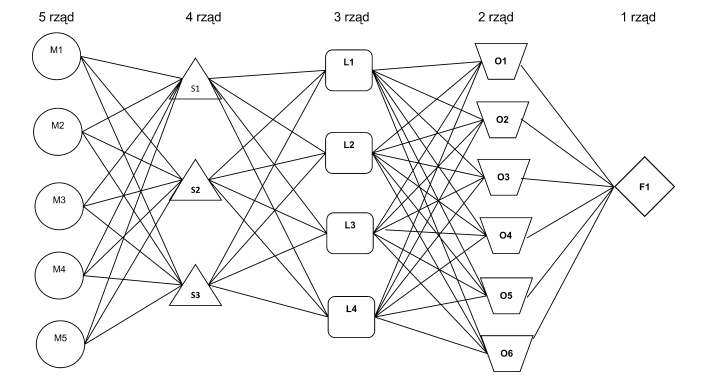
\includegraphics[width=\linewidth]{pictures/siec.png}

W tej pracy stosowane jest rozszerzenie tego podejścia, poprzez zaprogramowanie jako agentów jednostek przedsiębiorstwa (fabryka, magazyn, sklep, zarząd), które razem tworzą system (przedsiębiorstwo). Opiera się to na obserwacji, że relacje pomiędzy jednostkami w przedsiębiorstwie są analogiczne do relacji uczestników łańcucha dostaw. Michael Porter zauważył, że działalność przedsiębiorstwa to de facto sekwencja działań, która na każdym ogniwie zwiększa wartość dla odbiorcy. W przypadku firmy mamy więc również do czynienia z łańcuchem, który Micheal Porter określił jako łańcuch wartości (value chain).  Ponieważ przedsiębiorstwa często dysponują wieloma duplikującymi swoje działania jednostkami \footnote{Dobrym przykładem są tutaj zakłady samochodowe, które mogą produkować dany model w różnych krajach}, łańcuch ten jest nieliniowy i w jego przypadku mamy do czynienia z podobnymi wyzwaniami co w łańcuchu logistycznym.

Zdefiniowanie jako agentów poszczególnych jednostkek przedsiębiorstwa jest przy tym spójne z określoną przez Wooldridge i Jennings charakterystyką agenta, który według ich postulatów posiada : 
	\begin{itemize}
		\item autonomię - poszczególne jednostki przedsiębiorstwa podążają za strategią i celami narzuconymi przez zarząd, ale mają zazwyczaj swodobę w podejmowaniu decyzji dążących do ich realizacji
		\item zdolności do komunikacji - jednostki przedsiębiorstwa komunikują się z otoczeniem (relacje z klientami) oraz między sobą (raportowanie do zarządu, spotkania) i w ramach jednego przedsiębiorstwa występuje asymteria informacji pomiędzy jednostkami
		\item reaktywność - jednostki przedsiębiorstwa reagują na zmiany rynkowe oraz zmiany wewnętrz przedsiębiorstwa
	 	\item proaktywność - jednostki przedsiębiorstwa podejmują inicjatywy mające na celu zwiększyć wartość przedsiębiorstwa, jak działalność innowacyjna bądź ekspansja. 
	\end{itemize}

 

\bibliographystyle{plain}
\bibliography{bibliography}
\end{document}